%%%%%%%%%%%%
%
% $Autor: Wings $
% $Datum: 2019-03-05 08:03:15Z $
% $Pfad: SDCard $
% $Version: 4250 $
% !TeX spellcheck = en_GB/de_DE
% !TeX encoding = utf8
% !TeX root = filename 
% !TeX TXS-program:bibliography = txs:///biber
%
%%%%%%%%%%%%

\chapter{Arduino - SD-Karten-Modul}

Ein \ac{spi}-Lesegerät ist eine Art Modul, das die Kommunikation zwischen einem Mikrocontroller und einer Speicherkarte, z. B. einer \ac{sd}- oder \ac{tf}-Karte, ermöglicht. Das Modul verwendet das \ac{spi}-Protokoll, um Daten zwischen den beiden Geräten zu übertragen. Das \ac{sd}/\ac{tf}-Card-Shield-Modul ist ein spezieller Typ von \ac{spi}-Leser, der für die Verwendung mit Mikrocontroller-Boards konzipiert ist. Es ermöglicht einen einfachen Zugriff auf die auf der Speicherkarte gespeicherten Daten und kann für eine Vielzahl von Anwendungen wie Datenprotokollierung, Dateispeicherung und Multimedia-Projekte verwendet werden. Das Shield wird über die \ac{spi}-Schnittstelle mit dem Mikrocontroller verbunden.

\begin{figure}[h]
    \begin{center}
        
\includegraphics[width=12cm]{SDCard/SDCardSlot.png}
        \caption{SD/TF-Card-Shield-Modul}
        \label{fig:SD_Slot}
    \end{center}
\end{figure}

\section{Eigenschaften}

\begin{description}
    \item[Leichte und kostengünstige Erweiterung:] Der \ac{sd}-Karten Slot ermöglicht eine einfache und kostengünstige Erweiterung des Speicherplatzes für Ihr Arduino-Projekt mittels \ac{sd}-Karte.
    \item[Einfache Kommunikation:] Das Modul kommuniziert mit dem Mikrocontroller über das \ac{spi}-Protokoll, welches eine zuverlässige und schnelle Datenübertragung gewährleistet.
    \item[Unterstützung von Speicherkarten:] Es unterstützt sowohl Micro-SD-Karten (bis zu 2GB) als auch Micro-SDHC-Karten (bis zu 32GB), inklusive High-Speed-Karten.
    \item[Spannungsunterstützung:] Das Modul ist kompatibel mit einer Versorgungsspannung von 3,3-5V, was die Integration in verschiedene Projekte erleichtert.
\end{description}

\section{Technische Spezifikationen}

\begin{description}
    \item[Schnittstelle:] \ac{spi}
    \item[Unterstützte Karten:] Micro-SD-Karte (2GB), Micro-SDHC-Karte (bis zu 32GB)
    \item[Versorgungsspannung:] 3,3-5V
    \item[Kompatibilität:] Arduino und andere Mikrocontroller-Boards
\end{description}
\cite{AZ-Delivery:2021}



\section{Bibliothek \FILE{SD.h}}

Die SD.h Bibliothek ist eine essenzielle Bibliothek für Arduino-Entwickler, die es ermöglicht, \ac{sd}-Karten in ihren Projekten zu verwenden. Sie bietet eine einfache und effiziente Möglichkeit, Daten auf \ac{sd}-Karten zu speichern und zu lesen. Die Bibliothek unterstützt das FAT16 und FAT32 Dateisystem, was sie kompatibel mit den meisten \ac{sd}-Karten macht. Mit der SD.h Bibliothek können Dateien erstellt, gelöscht, umbenannt und bearbeitet werden. Zudem gibt es Funktionen zum Lesen und Schreiben von Daten in Dateien. Die Bibliothek ermöglicht das Erstellen und Löschen von Verzeichnissen (Ordnern) und unterstützt das Navigieren durch Verzeichnisse, was das Arbeiten mit komplexen Dateistrukturen erleichtert.

Die SD.h Bibliothek ist kompatibel mit den meisten Arduino-Boards, einschließlich Arduino Uno, Mega, Nano und anderen. Sie unterstützt sowohl Standard-\ac{sd}-Karten als auch microSD-Karten mit einem geeigneten Adapter. Die Integration der Bibliothek in Arduino-Sketches ist einfach und erfolgt durch leicht verständliche Methodenaufrufe. Die Arduino \ac{ide} enthält zudem Beispiele und umfangreiche Dokumentation, die den Einstieg in die Nutzung der SD.h Bibliothek erleichtern.


\section{Testen des SD-Karten Moduls}

Um das \ac{sd}-Karten Modul zu testen, haben wir ein Beispiel erstellt, das zeigt, wie man mit einem Arduino Daten auf einer \ac{sd}-Karte speichert und wieder ausliest. Basierend auf der Anleitung Funduino - Das \ac{sd}-Karten Modul haben wir den dortigen Beispielcode leicht angepasst \cite{AZ-Delivery:2021}. Zunächst wird die \ac{sd}-Karte initialisiert, um sicherzustellen, dass sie ordnungsgemäß funktioniert. Danach wird eine Testdatei erstellt, in die ein kurzer Text geschrieben wird. Anschließend wird der Inhalt dieser Datei ausgelesen und über den seriellen Monitor angezeigt.

\begin{code}[h]
    \pythonexternal[language=python]{../../Code/Arduino/SDCard/TestSDCard.ino}
    \caption{Testprogramm SD-Karten-Modul} 
    \label{Code:Test_SD_Karten_Modul}
\end{code}

\begin{center}
    
\includegraphics[width=10cm]{SDCard/SDCardTest}
    \captionof{figure}{Ausgabe SD-Kartentest Serieller Monitor}
    \label{fig:SD_Kartentest_Serieller_Monitor}	
\end{center}

\section{Entwicklerboard mit SD-Kartenleser}

Das \textit{Entwicklerboard mit SD-Kartenleser} \cite{AZDelivery.2024} ermöglicht eine einfache und kostengünstige Erweiterung des Arduino-Speicherplatzes durch einen integrierten Micro-SD-Kartenslot. Die Kommunikation mit dem Mikrocontroller erfolgt über das standardisierte SPI-Protokoll, was eine unkomplizierte Anbindung in bestehende Schaltungen erlaubt. Unterstützt werden sowohl Micro-SD-Karten mit einer Kapazität von bis zu 2 GB als auch Micro-SDHC-Karten mit bis zu 32 GB, einschließlich High-Speed-Karten. Der Betrieb des Moduls ist mit einer Versorgungsspannung von 3,3 - 5 V möglich, wodurch es direkt mit typischen Arduino-Boards kompatibel ist.

\bigskip

\begin{center}
    
\includegraphics[width=7cm]{SDCard/SDCardSlot}
    \captionof{figure}{SD-Kartenleser}
    \label{fig: SD-Kartenleser}
\end{center}

\textit{* Für eine ausgiebige Aktorbeschreibung siehe:} Kapitel \ref{sec:SDKartenleser}. 


\section{SD-Karte}

Die eingesetzte microSD-Karte des Herstellers \glqq SanDisk\grqq{} entspricht dem gängigen Formfaktor microSD und basiert auf dem UHS-I-Busstandard, der vollständig abwärtskompatibel zum SPI-Modus (vgl. Abschnitt~\ref{sec:SPI}) ist und somit eine problemlose Anbindung an das SD-Modul des Arduino Nano 33 BLE Sense Lite ermöglicht. Für eine zuverlässige Nutzung mit der Arduino-\texttt{SD}-Library wird eine Kapazität von 32\,GB gewählt. Dadurch kann das weit verbreitete FAT32-Dateisystem genutzt werden, das in Mikrocontroller-Anwendungen als De-facto-Standard gilt und Dateien bis zu einer Größe von 4\,GB unterstützt. Die maximale Übertragungsgeschwindigkeit der Karte beträgt laut Hersteller bis zu 120\,MB/s, wobei in SPI-Anwendungen niedrigere Übertragungsraten üblich sind. \cite{WesternDigitalTechnologies.2022}

Intern arbeitet die SD-Karte mit nichtflüchtigem NAND-Flash-Speicher, der durch einen integrierten Controller verwaltet wird. Dieser übernimmt Aufgaben wie Wear-Leveling, Fehlerkorrektur (ECC) und Adressumsetzung (LBA), wodurch der Mikrocontroller die Speicherkarte wie ein gewöhnliches Blockgerät ansprechen kann. Diese interne Abstraktion ermöglicht einen einfachen Zugriff auf Dateien über Bibliotheken wie \texttt{SD.h} oder \texttt{SdFat}. \cite{Subero.2024}

Obwohl der UHS-I-Standard primär für Hochgeschwindigkeitsübertragungen über den nativen SD-Bus vorgesehen ist, unterstützt die Karte weiterhin den SPI-Modus im sogenannten „Backward Compatibility Mode“. Wird die Initialisierung über SPI durchgeführt, erkennt die SD-Karte dies automatisch und wechselt in den SPI-kompatiblen Betriebsmodus. Dadurch kann die Karte auch in ressourcenbeschränkten Systemen zuverlässig betrieben werden, ohne dass ein spezialisierter SD-Controller erforderlich ist.

Die Versorgungsspannung der SD-Karte beträgt 3{,}3\,V. Da viele Mikrocontroller (z.\,B. Arduino Uno) jedoch mit 5\,V-Logikpegeln arbeiten, ist eine Pegelanpassung erforderlich. Das verwendete SD-Kartenmodul enthält hierfür integrierte Spannungsregler und Pegelwandler, wodurch die Karte sowohl mit 3{,}3\,V- als auch mit 5\,V-Systemen kompatibel ist.


Die eingesetzte microSD-Karte des Herstellers \glqq SanDisk\grqq{} entspricht dem gängigen Formfaktor microSD und basiert auf dem UHS-I-Busstandard, der vollständig abwärtskompatibel zum SPI-Modus ist und somit eine problemlose Anbindung an das SD-Modul des Arduino Nano 33 BLE Sense Lite ermöglicht. Für eine zuverlässige Nutzung mit der Arduino SD-Library wird eine Kapazität von 32 GB gewählt, dadurch wird das FAT32-Dateisystem mit maximalem Speicherplatz genutzt. Die Übertragungsgeschwindigkeit beträgt bis zu 120 MB/s.
\cite{WesternDigitalTechnologies.2022} 
\href{../../../Documents/Datenblaetter/Datenbatt SD-Karte}{[Datenblatt.PDF]}


Die folgende Tabelle zeigt die Pinbelegung einer MicroSD-Karte sowohl im standardmäßigen SD-Modus als auch im SPI-Modus, der typischerweise bei Mikrocontroller-Projekten zum Einsatz kommt. Die physikalische Anordnung der Kontakte ist in Abbildung~\ref{fig:SDKarte} dargestellt. \cite{KingstonTechnology.2022}

\begin{table}[H]
    \centering
    \begin{tabular}{|c|c|c|p{8cm}|}
        \hline
        \textbf{Pin} & \textbf{SD-Modus} & \textbf{SPI-Modus} & \textbf{Funktion} \\
        \hline
        1 & DAT2         & –                 & Datenleitung 2 (nur im 4-Bit SD-Modus aktiv, im SPI-Modus ungenutzt) \\
        2 & CD / DAT3    & CS (Chip Select)  & Chip-Select-Signal zur Auswahl der Karte im SPI-Bus \\
        3 & CMD          & DI (Data In)      & Kommandoleitung, überträgt Befehle vom Host zur Karte (MOSI) \\
        4 & VDD          & VDD               & Versorgungsspannung (typisch 3{,}3\,V) \\
        5 & CLK          & SCLK              & Taktleitung für die Datenübertragung \\
        6 & VSS          & VSS               & Masseanschluss (Ground) \\
        7 & DAT0         & DO (Data Out)     & Datenleitung 0, überträgt Daten von der Karte zum Host (MISO) \\
        8 & DAT1         & –                 & Datenleitung 1 (nur im 4-Bit SD-Modus aktiv, im SPI-Modus ungenutzt) \\
        \hline
    \end{tabular}
    \caption{Pinbelegung einer MicroSD-Karte im SD- und SPI-Modus}
    \label{tab:microSD_Pinbelegung}
\end{table}
\vspace{1ex}

\begin{center}
	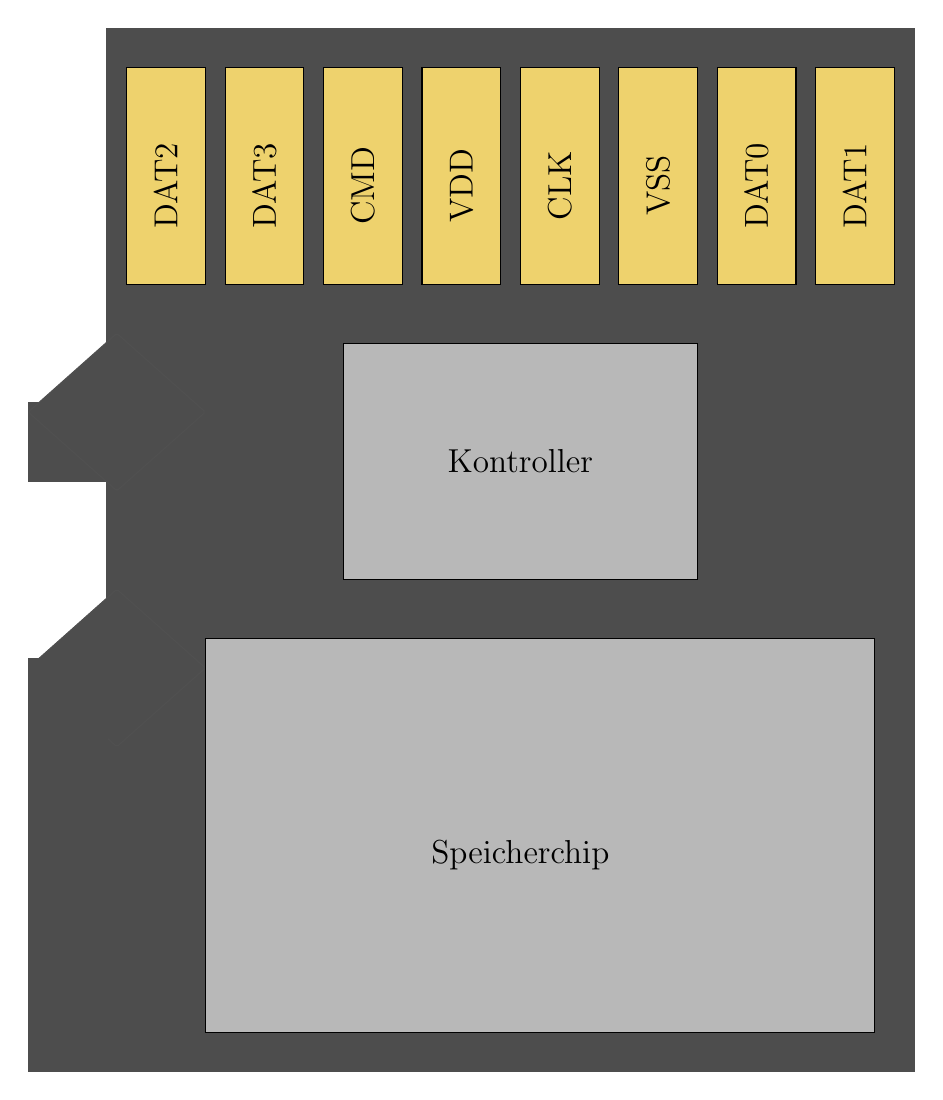
\begin{tikzpicture}		
    \draw [ color={rgb,255:red,77; green,77; blue,77} , fill={rgb,255:red,77; green,77; blue,77}] (16.25,17.5) rectangle (26.5,4.25);
    \draw [ color={rgb,255:red,80; green,80; blue,80} , fill={rgb,255:red,77; green,77; blue,77}, rounded corners = 0.6] (15.25,9.375) -- (16.375,8.375) -- (17.5,9.375) -- (16.375,10.375) -- cycle;
    \draw [ fill={rgb,255:red,238; green,210; blue,109} ] (16.5,17) rectangle (17.5,14.25);
    \node [font=\normalsize] at (17.5,16.25) {};
    \draw [ fill={rgb,255:red,238; green,210; blue,109} ] (17.75,17) rectangle (18.75,14.25);
    \draw [ color={rgb,255:red,77; green,77; blue,77} , fill={rgb,255:red,77; green,77; blue,77}] (15.25,9.5) rectangle (16.25,4.25);
    \draw [ color={rgb,255:red,77; green,77; blue,77} , fill={rgb,255:red,77; green,77; blue,77}] (15.25,12.75) rectangle (16.25,11.75);
    \draw [ color={rgb,255:red,80; green,80; blue,80} , fill={rgb,255:red,77; green,77; blue,77}, rounded corners = 0.6] (15.25,12.625) -- (16.375,11.625) -- (17.5,12.625) -- (16.375,13.625) -- cycle;
    \draw [ fill={rgb,255:red,238; green,210; blue,109} ] (19,17) rectangle (20,14.25);
    \draw [ fill={rgb,255:red,238; green,210; blue,109} ] (20.25,17) rectangle (21.25,14.25);
    \draw [ fill={rgb,255:red,238; green,210; blue,109} ] (21.5,17) rectangle (22.5,14.25);
    \draw [ fill={rgb,255:red,238; green,210; blue,109} ] (22.75,17) rectangle (23.75,14.25);
    \draw [ fill={rgb,255:red,238; green,210; blue,109} ] (24,17) rectangle (25,14.25);
    \node [font=\normalsize] at (22.75,15) {};
    \draw [ fill={rgb,255:red,238; green,210; blue,109} ] (25.25,17) rectangle (26.25,14.25);
    \draw [ fill={rgb,255:red,184; green,184; blue,184} ] (17.5,9.75) rectangle (26,4.75);
    \draw [ fill={rgb,255:red,184; green,184; blue,184} ] (19.25,13.5) rectangle (23.75,10.5);
    \node [font=\large] at (21.5,12) {Kontroller};
    \node [font=\large] at (21.5,7) {Speicherchip};
    \node [font=\large, rotate around={90:(0,0)}] at (17,15.5) {DAT2};
    \node [font=\large, rotate around={90:(0,0)}] at (18.25,15.5) {DAT3};
    \node [font=\large, rotate around={90:(0,0)}] at (19.5,15.5) {CMD};
    \node [font=\large, rotate around={90:(0,0)}] at (20.75,15.5) {VDD};
    \node [font=\large, rotate around={90:(0,0)}] at (22,15.5) {CLK};
    \node [font=\large, rotate around={90:(0,0)}] at (23.25,15.5) {VSS};
    \node [font=\large, rotate around={90:(0,0)}] at (24.5,15.5) {DAT0};
    \node [font=\large, rotate around={90:(0,0)}] at (25.75,15.5) {DAT1};
    
    
  \end{tikzpicture}
  \captionof{figure}{SD-Karte}
  \label{fig:SDKarte}
\end{center}

Im SPI-Modus sind nur vier Pins erforderlich:
\begin{itemize}
    \item \textbf{CS (Chip Select)} – Pin 2
    \item \textbf{MOSI (Data In)} – Pin 3
    \item \textbf{MISO (Data Out)} – Pin 7
    \item \textbf{SCK (Clock)} – Pin 5
\end{itemize}

Die übrigen Pins (DAT1, DAT2) bleiben im SPI-Betrieb ungenutzt. Die Versorgungsspannung liegt an Pin~4 (\textbf{VDD}), die Masseleitung an Pin~6 (\textbf{VSS}).


\begin{itemize}
    \item \textbf{CS (Chip Select) – Pin 2:}  
    Dient zur Auswahl des SD-Kartenmoduls im SPI-Bus. Wird vom Mikrocontroller auf \texttt{LOW} gezogen, um die Kommunikation mit der Karte zu aktivieren. Nur ein Gerät im SPI-Bus darf gleichzeitig ausgewählt sein.
    
    \item \textbf{MOSI (Master Out Slave In) – Pin 3:}  
    Überträgt Daten und Befehle vom Mikrocontroller (Master) zur SD-Karte (Slave). Dieser Pin wird im SD-Modus als \texttt{CMD} bezeichnet.
    
    \item \textbf{MISO (Master In Slave Out) – Pin 7:}  
    Überträgt Daten von der SD-Karte zum Mikrocontroller. Dieser Pin entspricht im SD-Modus der Leitung \texttt{DAT0}.
    
    \item \textbf{SCK (Serial Clock) – Pin 5:}  
    Liefert den Takt, mit dem die Datenübertragung im SPI-Protokoll synchronisiert wird. Der Takt wird vom Master (also vom Mikrocontroller) erzeugt.
\end{itemize}


\section{Entwicklerboard mit SD-Kartenleser}

Das \textit{Entwicklerboard mit SD-Kartenleser} \cite{AZDelivery.2024} ermöglicht eine Erweiterung des Arduino-Speicherplatzes durch einen integrierten Micro-SD-Kartenslot. Die Kommunikation mit dem Mikrocontroller erfolgt über das standardisierte SPI-Protokoll. Unterstützt werden sowohl Micro-SD-Karten mit einer Kapazität von bis zu 2 GB als auch Micro-SDHC-Karten mit bis zu 32 GB, einschließlich High-Speed-Karten. Der Betrieb des Moduls ist mit einer Versorgungsspannung von 3,3 - 5 V möglich.

\bigskip

\begin{center}
    
\includegraphics[width=7cm]{SDCard/SDCardSlot}
    \captionof{figure}{SD-Kartenleser}
    \label{fig: SD-Kartenleser}
\end{center}

\textit{* Für eine ausgiebige Aktorbeschreibung siehe:} Kapitel \ref{sec:SDKartenleser}. 


\section{SD-Karte}

Die eingesetzte microSD-Karte des Herstellers „SanDisk“ entspricht dem gängigen Formfaktor microSD und basiert auf dem UHS-I-Busstandard, der vollständig abwärtskompatibel zum SPI-Modus (vgl. Abschnitt~\ref{sec:SPI}) ist und somit eine problemlose Anbindung an das SD-Modul des Arduino Nano 33 BLE Sense Lite ermöglicht. Für eine zuverlässige Nutzung mit der Arduino-\texttt{SD}-Library wird eine Kapazität von 32\,GB gewählt. Dadurch kann das weit verbreitete FAT32-Dateisystem genutzt werden, das in Mikrocontroller-Anwendungen als De-facto-Standard gilt und Dateien bis zu einer Größe von 4\,GB unterstützt. Die maximale Übertragungsgeschwindigkeit der Karte beträgt laut Hersteller bis zu 120\,MB/s, wobei in SPI-Anwendungen niedrigere Übertragungsraten üblich sind. \cite{WesternDigitalTechnologies.2022}

Intern arbeitet die SD-Karte mit nichtflüchtigem NAND-Flash-Speicher, der durch einen integrierten Controller verwaltet wird. Dieser übernimmt Aufgaben wie Wear-Leveling, Fehlerkorrektur (ECC) und Adressumsetzung (LBA), wodurch der Mikrocontroller die Speicherkarte wie ein gewöhnliches Blockgerät ansprechen kann. Diese interne Abstraktion ermöglicht einen einfachen Zugriff auf Dateien über Bibliotheken wie \texttt{SD.h} oder \texttt{SdFat}. \cite{Subero.2024}

Obwohl der UHS-I-Standard primär für Hochgeschwindigkeitsübertragungen über den nativen SD-Bus vorgesehen ist, unterstützt die Karte weiterhin den SPI-Modus im sogenannten „Backward Compatibility Mode“. Wird die Initialisierung über SPI durchgeführt, erkennt die SD-Karte dies automatisch und wechselt in den SPI-kompatiblen Betriebsmodus. Dadurch kann die Karte auch in ressourcenbeschränkten Systemen zuverlässig betrieben werden, ohne dass ein spezialisierter SD-Controller erforderlich ist.

Die Versorgungsspannung der SD-Karte beträgt 3{,}3\,V. Da viele Mikrocontroller (z.\,B. Arduino Uno) jedoch mit 5\,V-Logikpegeln arbeiten, ist eine Pegelanpassung erforderlich. Das verwendete SD-Kartenmodul enthält hierfür integrierte Spannungsregler und Pegelwandler, wodurch die Karte sowohl mit 3{,}3\,V- als auch mit 5\,V-Systemen kompatibel ist.


Die eingesetzte microSD-Karte des Herstellers „SanDisk“ entspricht dem gängigen Formfaktor microSD und basiert auf dem UHS-I-Busstandard, der vollständig abwärtskompatibel zum SPI-Modus ist und somit eine problemlose Anbindung an das SD-Modul des Arduino Nano 33 BLE Sense Lite ermöglicht. Für eine zuverlässige Nutzung mit der Arduino SD-Library wird eine Kapazität von 32 GB gewählt, dadurch wird das FAT32-Dateisystem mit maximalem Speicherplatz genutzt. Die Übertragungsgeschwindigkeit beträgt bis zu 120 MB/s.
\cite{WesternDigitalTechnologies.2022} 
\href{../../../Documents/Datenblaetter/Datenbatt SD-Karte}{[Datenblatt.PDF]}


Die folgende Tabelle zeigt die Pinbelegung einer MicroSD-Karte sowohl im standardmäßigen SD-Modus als auch im SPI-Modus, der typischerweise bei Mikrocontroller-Projekten zum Einsatz kommt. Die physikalische Anordnung der Kontakte ist in Abbildung~\ref{fig:SDKarte} dargestellt. \cite{KingstonTechnology.2022}

\begin{center}
    \begin{tabular}{|c|c|c|p{8cm}|}
        \hline
        \textbf{Pin} & \textbf{SD-Modus} & \textbf{SPI-Modus} & \textbf{Funktion} \\
        \hline
        1 & DAT2         & –                 & Datenleitung 2 (nur im 4-Bit SD-Modus aktiv, im SPI-Modus ungenutzt) \\
        2 & CD / DAT3    & CS (Chip Select)  & Chip-Select-Signal zur Auswahl der Karte im SPI-Bus \\
        3 & CMD          & DI (Data In)      & Kommandoleitung, überträgt Befehle vom Host zur Karte (MOSI) \\
        4 & VDD          & VDD               & Versorgungsspannung (typisch 3{,}3\,V) \\
        5 & CLK          & SCLK              & Taktleitung für die Datenübertragung \\
        6 & VSS          & VSS               & Masseanschluss (Ground) \\
        7 & DAT0         & DO (Data Out)     & Datenleitung 0, überträgt Daten von der Karte zum Host (MISO) \\
        8 & DAT1         & –                 & Datenleitung 1 (nur im 4-Bit SD-Modus aktiv, im SPI-Modus ungenutzt) \\
        \hline
    \end{tabular}
    \captionof{table}{Pinbelegung einer MicroSD-Karte im SD- und SPI-Modus}
    \label{tab:microSD_Pinbelegung}
\end{center}

\bigskip

\begin{center}
	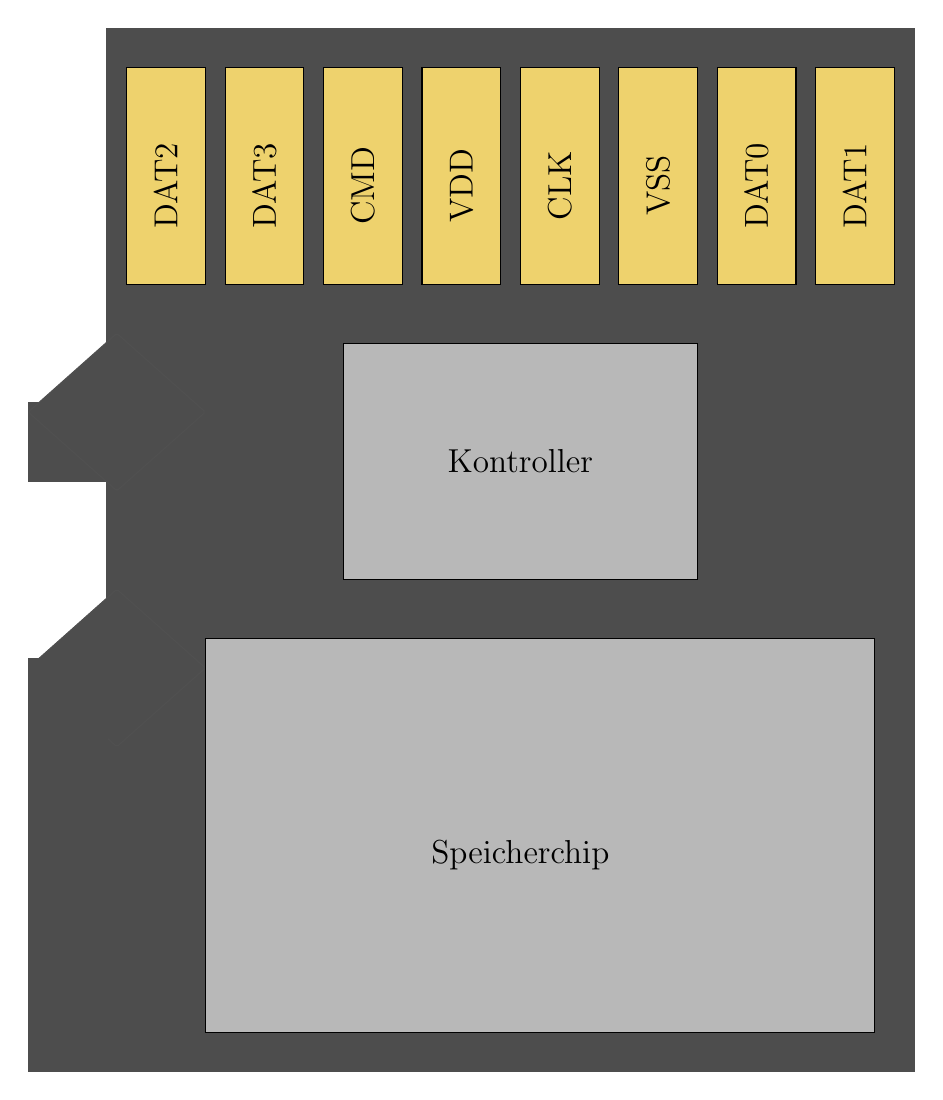
\begin{tikzpicture}		
    \draw [ color={rgb,255:red,77; green,77; blue,77} , fill={rgb,255:red,77; green,77; blue,77}] (16.25,17.5) rectangle (26.5,4.25);
    \draw [ color={rgb,255:red,80; green,80; blue,80} , fill={rgb,255:red,77; green,77; blue,77}, rounded corners = 0.6] (15.25,9.375) -- (16.375,8.375) -- (17.5,9.375) -- (16.375,10.375) -- cycle;
    \draw [ fill={rgb,255:red,238; green,210; blue,109} ] (16.5,17) rectangle (17.5,14.25);
    \node [font=\normalsize] at (17.5,16.25) {};
    \draw [ fill={rgb,255:red,238; green,210; blue,109} ] (17.75,17) rectangle (18.75,14.25);
    \draw [ color={rgb,255:red,77; green,77; blue,77} , fill={rgb,255:red,77; green,77; blue,77}] (15.25,9.5) rectangle (16.25,4.25);
    \draw [ color={rgb,255:red,77; green,77; blue,77} , fill={rgb,255:red,77; green,77; blue,77}] (15.25,12.75) rectangle (16.25,11.75);
    \draw [ color={rgb,255:red,80; green,80; blue,80} , fill={rgb,255:red,77; green,77; blue,77}, rounded corners = 0.6] (15.25,12.625) -- (16.375,11.625) -- (17.5,12.625) -- (16.375,13.625) -- cycle;
    \draw [ fill={rgb,255:red,238; green,210; blue,109} ] (19,17) rectangle (20,14.25);
    \draw [ fill={rgb,255:red,238; green,210; blue,109} ] (20.25,17) rectangle (21.25,14.25);
    \draw [ fill={rgb,255:red,238; green,210; blue,109} ] (21.5,17) rectangle (22.5,14.25);
    \draw [ fill={rgb,255:red,238; green,210; blue,109} ] (22.75,17) rectangle (23.75,14.25);
    \draw [ fill={rgb,255:red,238; green,210; blue,109} ] (24,17) rectangle (25,14.25);
    \node [font=\normalsize] at (22.75,15) {};
    \draw [ fill={rgb,255:red,238; green,210; blue,109} ] (25.25,17) rectangle (26.25,14.25);
    \draw [ fill={rgb,255:red,184; green,184; blue,184} ] (17.5,9.75) rectangle (26,4.75);
    \draw [ fill={rgb,255:red,184; green,184; blue,184} ] (19.25,13.5) rectangle (23.75,10.5);
    \node [font=\large] at (21.5,12) {Kontroller};
    \node [font=\large] at (21.5,7) {Speicherchip};
    \node [font=\large, rotate around={90:(0,0)}] at (17,15.5) {DAT2};
    \node [font=\large, rotate around={90:(0,0)}] at (18.25,15.5) {DAT3};
    \node [font=\large, rotate around={90:(0,0)}] at (19.5,15.5) {CMD};
    \node [font=\large, rotate around={90:(0,0)}] at (20.75,15.5) {VDD};
    \node [font=\large, rotate around={90:(0,0)}] at (22,15.5) {CLK};
    \node [font=\large, rotate around={90:(0,0)}] at (23.25,15.5) {VSS};
    \node [font=\large, rotate around={90:(0,0)}] at (24.5,15.5) {DAT0};
    \node [font=\large, rotate around={90:(0,0)}] at (25.75,15.5) {DAT1};
    
    
  \end{tikzpicture}
  \captionof{figure}{SD-Karte}
  \label{fig:SDKarte}
\end{center}

Im SPI-Modus sind nur vier Pins erforderlich:

\begin{itemize}
    \item \textbf{CS (Chip Select)} – Pin 2
    \item \textbf{MOSI (Data In)} – Pin 3
    \item \textbf{MISO (Data Out)} – Pin 7
    \item \textbf{SCK (Clock)} – Pin 5
\end{itemize}

Die übrigen Pins (DAT1, DAT2) bleiben im SPI-Betrieb ungenutzt. Die Versorgungsspannung liegt an Pin~4 (\textbf{VDD}), die Masseleitung an Pin~6 (\textbf{VSS}).


\begin{itemize}
    \item \textbf{CS (Chip Select) – Pin 2:}  
    Dient zur Auswahl des SD-Kartenmoduls im SPI-Bus. Wird vom Mikrocontroller auf \texttt{LOW} gezogen, um die Kommunikation mit der Karte zu aktivieren. Nur ein Gerät im SPI-Bus darf gleichzeitig ausgewählt sein.
    
    \item \textbf{MOSI (Master Out Slave In) – Pin 3:}  
    Überträgt Daten und Befehle vom Mikrocontroller (Master) zur SD-Karte (Slave). Dieser Pin wird im SD-Modus als \texttt{CMD} bezeichnet.
    
    \item \textbf{MISO (Master In Slave Out) – Pin 7:}  
    Überträgt Daten von der SD-Karte zum Mikrocontroller. Dieser Pin entspricht im SD-Modus der Leitung \texttt{DAT0}.
    
    \item \textbf{SCK (Serial Clock) – Pin 5:}  
    Liefert den Takt, mit dem die Datenübertragung im SPI-Protokoll synchronisiert wird. Der Takt wird vom Master (also vom Mikrocontroller) erzeugt.
\end{itemize}


\chapter{SD-Karten-Modul}\label{SD-Karten-Modul}


Ein \ac{spi}-Lesegerät ist ein Modul, das die Kommunikation zwischen einem Mikrocontroller und einer Speicherkarte, z. B. einer \ac{sd}- oder \ac{tf}-Karte, ermöglicht. Das Modul verwendet das \ac{spi}-Protokoll, um Daten zwischen den beiden Geräten zu übertragen. Das \ac{sd}/\ac{tf}-Card-Shield-Modul ist ein spezieller Typ von \ac{spi}-Leser, der für die Verwendung mit Mikrocontroller-Boards konzipiert ist. Es ermöglicht den Zugriff auf gespeicherte Daten auf der SD-Karte und kann für eine Vielzahl von Anwendungen wie Datenprotokollierung, Dateispeicherung und Multimedia-Projekte verwendet werden. Das Shield wird über die \ac{spi}-Schnittstelle mit dem Mikrocontroller verbunden(Abbildung~\ref{fig:SD_Slot}).\cite{AZDelivery2025}

Ein \ac{spi}-Lesegerät ist eine Art Modul, das die Kommunikation zwischen einem Mikrocontroller und einer Speicherkarte, z. B. einer \ac{sd}- oder \ac{tf}-Karte, ermöglicht. Das Modul verwendet das \ac{spi}-Protokoll, um Daten zwischen den beiden Geräten zu übertragen. Das \ac{sd}/\ac{tf}-Card-Shield-Modul ist ein spezieller Typ von \ac{spi}-Leser, der für die Verwendung mit Mikrocontroller-Boards konzipiert ist. Es ermöglicht einen einfachen Zugriff auf die auf der Speicherkarte gespeicherten Daten und kann für eine Vielzahl von Anwendungen wie Datenprotokollierung, Dateispeicherung und Multimedia-Projekte verwendet werden. Das Shield wird über die \ac{spi}-Schnittstelle mit dem Mikrocontroller verbunden(Abbilung~\ref{fig:SD_Slot}).\cite{AZDelivery2025}

\begin{center}
	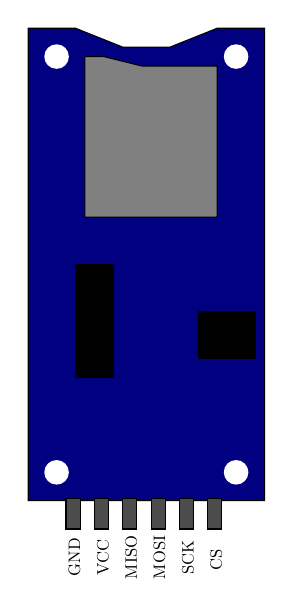
\begin{tikzpicture}[scale=1.2]
		% Vergrößerte Platine
		\filldraw [fill=blue!50!black](0,0) -- (0,5)--(0.5,5)--(1,4.8)--(1.5,4.8)--(2,5)--(2.5,5)--(2.5,0)--cycle;
		\filldraw [fill=black!50](0.6,3) -- (0.6,4.7)--(0.8,4.7)--(1.2,4.6)--(2,4.6)--(2,3)--cycle;
		\filldraw [fill=black!120](1.8,1.5) -- (1.8,2)-- (2.4,2)--(2.4,1.5)--cycle;
		\filldraw [fill=black!100](0.5,1.3) -- (0.5,2.5)-- (0.9,2.5)--(0.9,1.3)--cycle;
		% Bohrlöcher
		\foreach \x/\y in {0.3/0.3, 0.3/4.7, 2.2/4.7, 2.2/0.3} {
			\fill [white] (\x,\y) circle (0.13);
		}
		\foreach \i/\name in {
			0/GND,
			1/VCC,
			2/MISO,
			3/MOSI,
			4/SCK,
			5/CS
		} { 
			\pgfmathsetmacro\y{0.1 -\i * 0.3}
			\filldraw[fill=black!70] ( 0.5-\y,-0.3) rectangle +(0.15, 0.32);
			\node[anchor=center, text=black, rotate=90] at (0.59-\y, -0.6) {\scalebox{0.6}{\name}};
		}
	\end{tikzpicture}
	\captionof{figure}{SD-Karten-Modul nach \cite{funduinoSD2025} }
	\label{fig:SD_Slot}
\end{center}

\section{Eigenschaften}

\begin{description}
	\item[Leichte und kostengünstige Erweiterung:] Der \ac{sd}-Karten-Slot ermöglicht eine einfache und kostengünstige Erweiterung des Speicherplatzes für Ihr Arduino-Projekt mittels \ac{sd}-Karte.
	\item[Einfache Kommunikation:] Das Modul kommuniziert mit dem Mikrocontroller über das \ac{spi}-Protokoll, welches eine zuverlässige und schnelle Datenübertragung gewährleistet.
	\item[Unterstützung von Speicherkarten:] Es unterstützt sowohl Micro-SD-Karten (bis zu 2~~GB) als auch Micro-SDHC-Karten (bis zu 32~GB), inklusive High-Speed-Karten.
	\item[Spannungsunterstützung:] Das Modul ist kompatibel mit einer Versorgungsspannung von 3,3-5V, was die Integration in verschiedene Projekte erleichtert.\cite{AZDelivery2025}
\end{description}

\section{Technische Spezifikationen}

Dies ist in der folgenden Tabelle \ref{tab:Technische Spezifikationen} dargestellt. Für das Projekt Schlüsselkasten ist insbesondere die 3.3~V Kompatibilität entscheidend.

\begin{center}
	\captionof{table}{Technische Spezifikationen: SD-Karten-Modul  	\cite{funduinoSD2025}}\label{tab:Technische Spezifikationen}
	\begin{tabular}{|l|l|}
		
		\hline
		Schnittstelle&\ac{spi} \\
		\hline
		Unterstützte Karten& Micro-SD-Karte (2\,GB), Micro-SDHC-Karte (bis zu 32GB) \\
		\hline
		Versorgungsspannung& 3,3-5~V \\
		\hline
		Kompatibilität&  Arduino und andere Mikrocontroller-Boards  \\
		\hline
	\end{tabular}
\end{center}


\section{Bibliothek \FILE{SD.h}}


Die \PYTHON{SD.h} Bibliothek ist eine Bibliothek für Arduino-Entwickler, die es ermöglicht, \ac{sd}-Karten in ihren Projekten zu verwenden. Sie bietet eine einfache und effiziente Methode, Daten auf \ac{sd}-Karten zu speichern und zu lesen. Die Bibliothek unterstützt das FAT16 und FAT32 Dateisystem, was sie kompatibel mit den meisten \ac{sd}-Karten macht. Mit der \PYTHON{SD.h} Bibliothek können Dateien erstellt, gelöscht, umbenannt und bearbeitet werden. Zudem gibt es Funktionen zum Lesen und Schreiben von Daten in Dateien. Die Bibliothek ermöglicht das Erstellen und Löschen von Verzeichnissen (Ordnern) und unterstützt das Navigieren durch Verzeichnisse, was das Arbeiten mit komplexen Dateistrukturen erleichtert.



\section{Testen des SD-Karten-Moduls}

Um das \ac{sd}-Karten Modul zu testen, haben wir ein Beispiel erstellt(Listing~\ref{Code:Test_SD_Karten_Modul}), das zeigt, wie man mit einem Arduino Daten auf einer \ac{sd}-Karte speichert und wieder ausliest. Basierend auf der Anleitung Funduino - Das \ac{sd}-Karten Modul haben wir den dortigen Beispielcode leicht angepasst \cite{AZDelivery2025}. Zunächst wird die \ac{sd}-Karte initialisiert, um sicherzustellen, dass sie ordnungsgemäß funktioniert. Danach wird eine Testdatei erstellt, in die ein kurzer Text geschrieben wird. Anschließend wird der Inhalt dieser Datei ausgelesen und über den seriellen Monitor angezeigt (Abbilung~\ref{fig:SD_Kartentest_Serieller_Monitor}).

\subsection{Anschluss am Tiny Machine Learning Shield}
Die Pins GND und 3.3~V werden später an die Grove Schnittstelle angeschlossen, da diese für den RFID-Sensor verwendet werden. Für den ersten Test werden die Pins wie in Abbildung \ref{fig:pins_shield_SD} beschrieben angeschlossen. Bei den Pins handelt es sich um digitale Pins, diese sind aus dem Schaltplans des Tiny Machine Learning Shields \ref{fig:TML_Cam} zu entnehmen. 


\begin{center}
	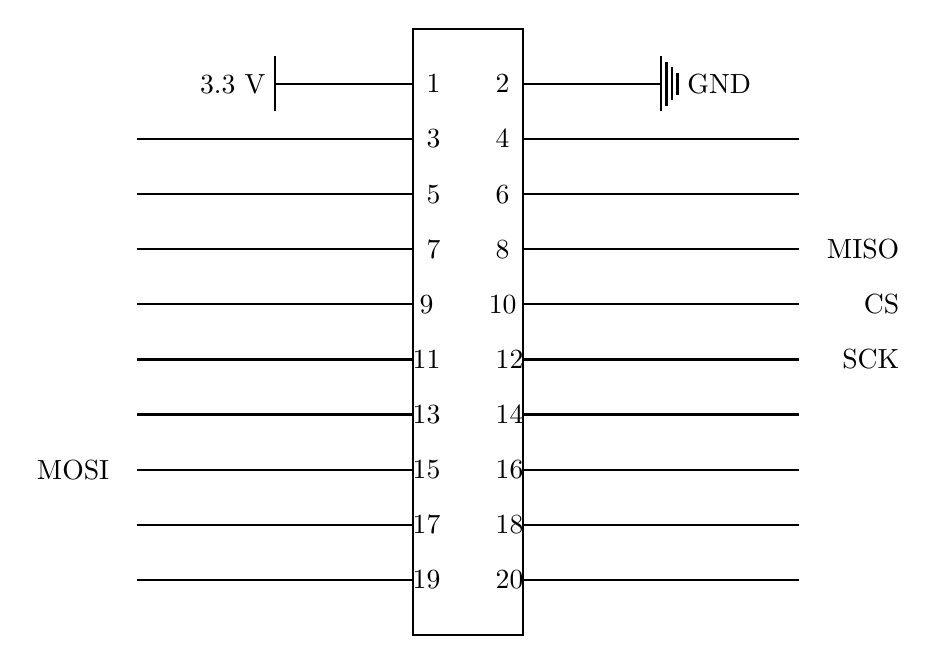
\begin{tikzpicture}[scale=0.7]
		% Rechteck
		\draw[thick] (5, 0) rectangle (7, 11);
		
		% Linien mit Beschriftung und Innenbeschriftung
		\foreach \y/\leftlabel/\rightlabel/\leftdesc/\rightdesc in {
			1/19/20//,
			2/17/18//,
			3/15/16/MOSI/,
			4/13/14//,
			5/11/12//SCK,
			6/9/10//CS,
			7/7/8//MISO,
			8/5/6//,
			9/3/4//,
			10/1/2/ /
		} {
			% Sonderfall: 3 V (Linie 10)
			\ifnum\y=10
			\draw[thick] (2.5,\y) -- (5,\y); % linke Linie gekürzt
			\node[anchor=center] at (6,\y) {\leftlabel\quad\quad\rightlabel}; % Rechteck-Beschriftung
			\node[anchor=west] at (2.5,\y) {\leftdesc}; % Beschreibung links
			\node[anchor=east] at (9.5,\y) {\rightdesc}; % Beschreibung rechts
			\draw[thick] (2.5,9.5) -- (2.5,10.5); % senkrechte 3V Linie
			\node[left] at (2.5, 10) {3.3~V};
			\draw[thick] (9.5,9.5) -- (9.5,10.5); % GND Linie
			\draw[thick] (9.6,9.6) -- (9.6,10.4);
			\draw[thick] (9.7,9.7) -- (9.7,10.3);
			\draw[thick] (9.8,9.8) -- (9.8,10.2);
			\node[right] at (9.8, 10) {GND};
			\draw[thick] (7,\y) -- (9.5,\y); % rechte Linie ganz
			% Sonderfall: GND (Linie 9)
			\else\ifnum\y=9
			% Sonderfall GND hier behandeln (falls benötigt)
			\draw[thick] (0,\y) -- (5,\y); % linke Linie
			\draw[thick] (7,\y) -- (12,\y); % rechte Linie
			\node[anchor=center] at (6,\y) {\leftlabel\quad\quad\rightlabel}; % Zahlen im Rechteck
			\node[anchor=west] at (-1,\y) {\leftdesc}; % Beschreibung links
			\node[anchor=east] at (13,\y) {\rightdesc}; % Beschreibung rechts
			% Alle anderen Pins
			\else
			\draw[thick] (0,\y) -- (5,\y); % linke Linie
			\draw[thick] (7,\y) -- (12,\y); % rechte Linie
			% Zahlen im Rechteck (weiter auseinander)
			\node[anchor=center] at (6,\y) {\leftlabel\quad\quad\rightlabel}; % Zahlen im Rechteck
			\node[anchor=west] at (-2,\y) {\leftdesc}; % Beschreibung links
			\node[anchor=east] at (14,\y) {\rightdesc}; % Beschreibung rechts
			\fi\fi
		}
	\end{tikzpicture}
	\captionof{figure}{Pins des Shields nach  \cite{ArduinoShield:2021} und \ref{TinyMachineLearningShieldPins}\label{fig:pins_shield_SD}}
\end{center}

\subsection{Testprogramm des SD-Karten Moduls}

{
	\captionof{code}{Testprogramm für das SD-Karten-Modul} 
	\label{Code:Test_SD_Karten_Modul}
	\ArduinoExternal{}{../../Code/Arduino/SDCard/TestSDCard/TestSDCard.ino}
	
}

\begin{center}
	
\includegraphics[width=10cm]{SDCard/SDCardTest}
	\captionof{figure}{Ausgabe SD-Kartentest Serieller Monitor [eigene Darstellung]}
	\label{fig:SD_Kartentest_Serieller_Monitor}	
\end{center}
